\section{Experimental setup}
% The current experiment is still being discussed, however the infrastructure allows us to test two different phishing detection models and then utilize metrics such as the average rate of phishing detected and the average phishing probability returned by the model. The current model-service endpoints does not yet support predictions with known feature-label pairs so it is not yet possible to determine metrics such as accuracy. An example hypothesis that can currently be tested could be: \textit{A model trained on fewer epochs is more likely to predict "legitimate" and therefore has a lower average phishing rate.}
The experiment is to use the capability of canary releases in order to test 2 different models. The first model was trained for 2 epochs while the other model is trained for 5 epochs. The hypothesis is that the model trained on more epochs has a better accuracy. In order to evaluate this the model\_accuracy metric is collected. To do this experiment we release two different versions of the model-service image. The v1 model-service deployment is set to serve the 2 epoch model while the v2 model-service deployment serves the 5 epoch model. To evaluate the result Prometheus can be queried for model\_accuracy or the Grafana dashboard can be used instead as seen in \autoref{fig:grafana}.

\begin{figure}[ht!]
    \centering
    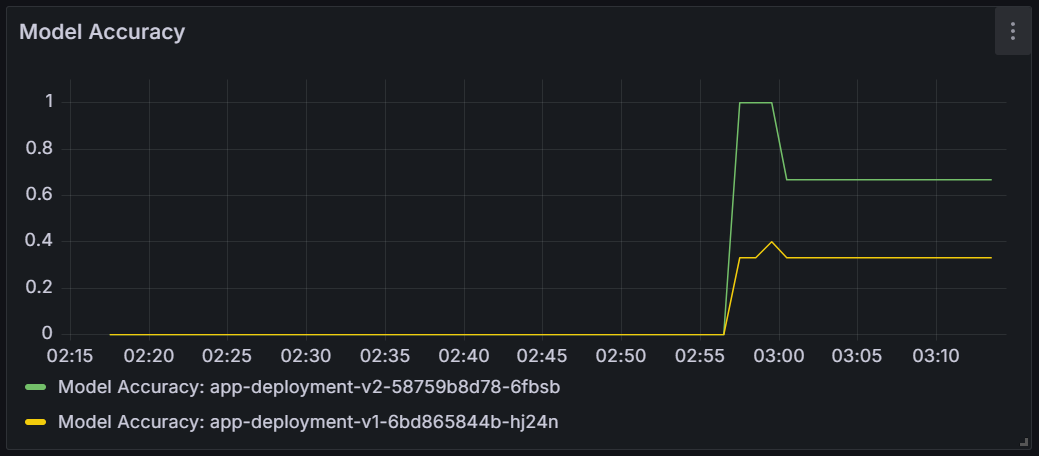
\includegraphics[width=8.5cm]{report/images/grafana.png}
    \caption{Grafana dashboard for model accuracy}
    \label{fig:grafana}
\end{figure}